
% Default to the notebook output style

    


% Inherit from the specified cell style.




    
\documentclass[11pt]{article}

    
    
    \usepackage[T1]{fontenc}
    % Nicer default font (+ math font) than Computer Modern for most use cases
    \usepackage{mathpazo}

    % Basic figure setup, for now with no caption control since it's done
    % automatically by Pandoc (which extracts ![](path) syntax from Markdown).
    \usepackage{graphicx}
    % We will generate all images so they have a width \maxwidth. This means
    % that they will get their normal width if they fit onto the page, but
    % are scaled down if they would overflow the margins.
    \makeatletter
    \def\maxwidth{\ifdim\Gin@nat@width>\linewidth\linewidth
    \else\Gin@nat@width\fi}
    \makeatother
    \let\Oldincludegraphics\includegraphics
    % Set max figure width to be 80% of text width, for now hardcoded.
    \renewcommand{\includegraphics}[1]{\Oldincludegraphics[width=.8\maxwidth]{#1}}
    % Ensure that by default, figures have no caption (until we provide a
    % proper Figure object with a Caption API and a way to capture that
    % in the conversion process - todo).
    \usepackage{caption}
    \DeclareCaptionLabelFormat{nolabel}{}
    \captionsetup{labelformat=nolabel}

    \usepackage{adjustbox} % Used to constrain images to a maximum size 
    \usepackage{xcolor} % Allow colors to be defined
    \usepackage{enumerate} % Needed for markdown enumerations to work
    \usepackage{geometry} % Used to adjust the document margins
    \usepackage{amsmath} % Equations
    \usepackage{amssymb} % Equations
    \usepackage{textcomp} % defines textquotesingle
    % Hack from http://tex.stackexchange.com/a/47451/13684:
    \AtBeginDocument{%
        \def\PYZsq{\textquotesingle}% Upright quotes in Pygmentized code
    }
    \usepackage{upquote} % Upright quotes for verbatim code
    \usepackage{eurosym} % defines \euro
    \usepackage[mathletters]{ucs} % Extended unicode (utf-8) support
    \usepackage[utf8x]{inputenc} % Allow utf-8 characters in the tex document
    \usepackage{fancyvrb} % verbatim replacement that allows latex
    \usepackage{grffile} % extends the file name processing of package graphics 
                         % to support a larger range 
    % The hyperref package gives us a pdf with properly built
    % internal navigation ('pdf bookmarks' for the table of contents,
    % internal cross-reference links, web links for URLs, etc.)
    \usepackage{hyperref}
    \usepackage{longtable} % longtable support required by pandoc >1.10
    \usepackage{booktabs}  % table support for pandoc > 1.12.2
    \usepackage[inline]{enumitem} % IRkernel/repr support (it uses the enumerate* environment)
    \usepackage[normalem]{ulem} % ulem is needed to support strikethroughs (\sout)
                                % normalem makes italics be italics, not underlines
    

    
    
    % Colors for the hyperref package
    \definecolor{urlcolor}{rgb}{0,.145,.698}
    \definecolor{linkcolor}{rgb}{.71,0.21,0.01}
    \definecolor{citecolor}{rgb}{.12,.54,.11}

    % ANSI colors
    \definecolor{ansi-black}{HTML}{3E424D}
    \definecolor{ansi-black-intense}{HTML}{282C36}
    \definecolor{ansi-red}{HTML}{E75C58}
    \definecolor{ansi-red-intense}{HTML}{B22B31}
    \definecolor{ansi-green}{HTML}{00A250}
    \definecolor{ansi-green-intense}{HTML}{007427}
    \definecolor{ansi-yellow}{HTML}{DDB62B}
    \definecolor{ansi-yellow-intense}{HTML}{B27D12}
    \definecolor{ansi-blue}{HTML}{208FFB}
    \definecolor{ansi-blue-intense}{HTML}{0065CA}
    \definecolor{ansi-magenta}{HTML}{D160C4}
    \definecolor{ansi-magenta-intense}{HTML}{A03196}
    \definecolor{ansi-cyan}{HTML}{60C6C8}
    \definecolor{ansi-cyan-intense}{HTML}{258F8F}
    \definecolor{ansi-white}{HTML}{C5C1B4}
    \definecolor{ansi-white-intense}{HTML}{A1A6B2}

    % commands and environments needed by pandoc snippets
    % extracted from the output of `pandoc -s`
    \providecommand{\tightlist}{%
      \setlength{\itemsep}{0pt}\setlength{\parskip}{0pt}}
    \DefineVerbatimEnvironment{Highlighting}{Verbatim}{commandchars=\\\{\}}
    % Add ',fontsize=\small' for more characters per line
    \newenvironment{Shaded}{}{}
    \newcommand{\KeywordTok}[1]{\textcolor[rgb]{0.00,0.44,0.13}{\textbf{{#1}}}}
    \newcommand{\DataTypeTok}[1]{\textcolor[rgb]{0.56,0.13,0.00}{{#1}}}
    \newcommand{\DecValTok}[1]{\textcolor[rgb]{0.25,0.63,0.44}{{#1}}}
    \newcommand{\BaseNTok}[1]{\textcolor[rgb]{0.25,0.63,0.44}{{#1}}}
    \newcommand{\FloatTok}[1]{\textcolor[rgb]{0.25,0.63,0.44}{{#1}}}
    \newcommand{\CharTok}[1]{\textcolor[rgb]{0.25,0.44,0.63}{{#1}}}
    \newcommand{\StringTok}[1]{\textcolor[rgb]{0.25,0.44,0.63}{{#1}}}
    \newcommand{\CommentTok}[1]{\textcolor[rgb]{0.38,0.63,0.69}{\textit{{#1}}}}
    \newcommand{\OtherTok}[1]{\textcolor[rgb]{0.00,0.44,0.13}{{#1}}}
    \newcommand{\AlertTok}[1]{\textcolor[rgb]{1.00,0.00,0.00}{\textbf{{#1}}}}
    \newcommand{\FunctionTok}[1]{\textcolor[rgb]{0.02,0.16,0.49}{{#1}}}
    \newcommand{\RegionMarkerTok}[1]{{#1}}
    \newcommand{\ErrorTok}[1]{\textcolor[rgb]{1.00,0.00,0.00}{\textbf{{#1}}}}
    \newcommand{\NormalTok}[1]{{#1}}
    
    % Additional commands for more recent versions of Pandoc
    \newcommand{\ConstantTok}[1]{\textcolor[rgb]{0.53,0.00,0.00}{{#1}}}
    \newcommand{\SpecialCharTok}[1]{\textcolor[rgb]{0.25,0.44,0.63}{{#1}}}
    \newcommand{\VerbatimStringTok}[1]{\textcolor[rgb]{0.25,0.44,0.63}{{#1}}}
    \newcommand{\SpecialStringTok}[1]{\textcolor[rgb]{0.73,0.40,0.53}{{#1}}}
    \newcommand{\ImportTok}[1]{{#1}}
    \newcommand{\DocumentationTok}[1]{\textcolor[rgb]{0.73,0.13,0.13}{\textit{{#1}}}}
    \newcommand{\AnnotationTok}[1]{\textcolor[rgb]{0.38,0.63,0.69}{\textbf{\textit{{#1}}}}}
    \newcommand{\CommentVarTok}[1]{\textcolor[rgb]{0.38,0.63,0.69}{\textbf{\textit{{#1}}}}}
    \newcommand{\VariableTok}[1]{\textcolor[rgb]{0.10,0.09,0.49}{{#1}}}
    \newcommand{\ControlFlowTok}[1]{\textcolor[rgb]{0.00,0.44,0.13}{\textbf{{#1}}}}
    \newcommand{\OperatorTok}[1]{\textcolor[rgb]{0.40,0.40,0.40}{{#1}}}
    \newcommand{\BuiltInTok}[1]{{#1}}
    \newcommand{\ExtensionTok}[1]{{#1}}
    \newcommand{\PreprocessorTok}[1]{\textcolor[rgb]{0.74,0.48,0.00}{{#1}}}
    \newcommand{\AttributeTok}[1]{\textcolor[rgb]{0.49,0.56,0.16}{{#1}}}
    \newcommand{\InformationTok}[1]{\textcolor[rgb]{0.38,0.63,0.69}{\textbf{\textit{{#1}}}}}
    \newcommand{\WarningTok}[1]{\textcolor[rgb]{0.38,0.63,0.69}{\textbf{\textit{{#1}}}}}
    
    
    % Define a nice break command that doesn't care if a line doesn't already
    % exist.
    \def\br{\hspace*{\fill} \\* }
    % Math Jax compatability definitions
    \def\gt{>}
    \def\lt{<}
    % Document parameters
    \title{Complex Networds: exercise 6 \\ Adam Ilyas 725819}
    
    
    

    % Pygments definitions
    
\makeatletter
\def\PY@reset{\let\PY@it=\relax \let\PY@bf=\relax%
    \let\PY@ul=\relax \let\PY@tc=\relax%
    \let\PY@bc=\relax \let\PY@ff=\relax}
\def\PY@tok#1{\csname PY@tok@#1\endcsname}
\def\PY@toks#1+{\ifx\relax#1\empty\else%
    \PY@tok{#1}\expandafter\PY@toks\fi}
\def\PY@do#1{\PY@bc{\PY@tc{\PY@ul{%
    \PY@it{\PY@bf{\PY@ff{#1}}}}}}}
\def\PY#1#2{\PY@reset\PY@toks#1+\relax+\PY@do{#2}}

\expandafter\def\csname PY@tok@w\endcsname{\def\PY@tc##1{\textcolor[rgb]{0.73,0.73,0.73}{##1}}}
\expandafter\def\csname PY@tok@c\endcsname{\let\PY@it=\textit\def\PY@tc##1{\textcolor[rgb]{0.25,0.50,0.50}{##1}}}
\expandafter\def\csname PY@tok@cp\endcsname{\def\PY@tc##1{\textcolor[rgb]{0.74,0.48,0.00}{##1}}}
\expandafter\def\csname PY@tok@k\endcsname{\let\PY@bf=\textbf\def\PY@tc##1{\textcolor[rgb]{0.00,0.50,0.00}{##1}}}
\expandafter\def\csname PY@tok@kp\endcsname{\def\PY@tc##1{\textcolor[rgb]{0.00,0.50,0.00}{##1}}}
\expandafter\def\csname PY@tok@kt\endcsname{\def\PY@tc##1{\textcolor[rgb]{0.69,0.00,0.25}{##1}}}
\expandafter\def\csname PY@tok@o\endcsname{\def\PY@tc##1{\textcolor[rgb]{0.40,0.40,0.40}{##1}}}
\expandafter\def\csname PY@tok@ow\endcsname{\let\PY@bf=\textbf\def\PY@tc##1{\textcolor[rgb]{0.67,0.13,1.00}{##1}}}
\expandafter\def\csname PY@tok@nb\endcsname{\def\PY@tc##1{\textcolor[rgb]{0.00,0.50,0.00}{##1}}}
\expandafter\def\csname PY@tok@nf\endcsname{\def\PY@tc##1{\textcolor[rgb]{0.00,0.00,1.00}{##1}}}
\expandafter\def\csname PY@tok@nc\endcsname{\let\PY@bf=\textbf\def\PY@tc##1{\textcolor[rgb]{0.00,0.00,1.00}{##1}}}
\expandafter\def\csname PY@tok@nn\endcsname{\let\PY@bf=\textbf\def\PY@tc##1{\textcolor[rgb]{0.00,0.00,1.00}{##1}}}
\expandafter\def\csname PY@tok@ne\endcsname{\let\PY@bf=\textbf\def\PY@tc##1{\textcolor[rgb]{0.82,0.25,0.23}{##1}}}
\expandafter\def\csname PY@tok@nv\endcsname{\def\PY@tc##1{\textcolor[rgb]{0.10,0.09,0.49}{##1}}}
\expandafter\def\csname PY@tok@no\endcsname{\def\PY@tc##1{\textcolor[rgb]{0.53,0.00,0.00}{##1}}}
\expandafter\def\csname PY@tok@nl\endcsname{\def\PY@tc##1{\textcolor[rgb]{0.63,0.63,0.00}{##1}}}
\expandafter\def\csname PY@tok@ni\endcsname{\let\PY@bf=\textbf\def\PY@tc##1{\textcolor[rgb]{0.60,0.60,0.60}{##1}}}
\expandafter\def\csname PY@tok@na\endcsname{\def\PY@tc##1{\textcolor[rgb]{0.49,0.56,0.16}{##1}}}
\expandafter\def\csname PY@tok@nt\endcsname{\let\PY@bf=\textbf\def\PY@tc##1{\textcolor[rgb]{0.00,0.50,0.00}{##1}}}
\expandafter\def\csname PY@tok@nd\endcsname{\def\PY@tc##1{\textcolor[rgb]{0.67,0.13,1.00}{##1}}}
\expandafter\def\csname PY@tok@s\endcsname{\def\PY@tc##1{\textcolor[rgb]{0.73,0.13,0.13}{##1}}}
\expandafter\def\csname PY@tok@sd\endcsname{\let\PY@it=\textit\def\PY@tc##1{\textcolor[rgb]{0.73,0.13,0.13}{##1}}}
\expandafter\def\csname PY@tok@si\endcsname{\let\PY@bf=\textbf\def\PY@tc##1{\textcolor[rgb]{0.73,0.40,0.53}{##1}}}
\expandafter\def\csname PY@tok@se\endcsname{\let\PY@bf=\textbf\def\PY@tc##1{\textcolor[rgb]{0.73,0.40,0.13}{##1}}}
\expandafter\def\csname PY@tok@sr\endcsname{\def\PY@tc##1{\textcolor[rgb]{0.73,0.40,0.53}{##1}}}
\expandafter\def\csname PY@tok@ss\endcsname{\def\PY@tc##1{\textcolor[rgb]{0.10,0.09,0.49}{##1}}}
\expandafter\def\csname PY@tok@sx\endcsname{\def\PY@tc##1{\textcolor[rgb]{0.00,0.50,0.00}{##1}}}
\expandafter\def\csname PY@tok@m\endcsname{\def\PY@tc##1{\textcolor[rgb]{0.40,0.40,0.40}{##1}}}
\expandafter\def\csname PY@tok@gh\endcsname{\let\PY@bf=\textbf\def\PY@tc##1{\textcolor[rgb]{0.00,0.00,0.50}{##1}}}
\expandafter\def\csname PY@tok@gu\endcsname{\let\PY@bf=\textbf\def\PY@tc##1{\textcolor[rgb]{0.50,0.00,0.50}{##1}}}
\expandafter\def\csname PY@tok@gd\endcsname{\def\PY@tc##1{\textcolor[rgb]{0.63,0.00,0.00}{##1}}}
\expandafter\def\csname PY@tok@gi\endcsname{\def\PY@tc##1{\textcolor[rgb]{0.00,0.63,0.00}{##1}}}
\expandafter\def\csname PY@tok@gr\endcsname{\def\PY@tc##1{\textcolor[rgb]{1.00,0.00,0.00}{##1}}}
\expandafter\def\csname PY@tok@ge\endcsname{\let\PY@it=\textit}
\expandafter\def\csname PY@tok@gs\endcsname{\let\PY@bf=\textbf}
\expandafter\def\csname PY@tok@gp\endcsname{\let\PY@bf=\textbf\def\PY@tc##1{\textcolor[rgb]{0.00,0.00,0.50}{##1}}}
\expandafter\def\csname PY@tok@go\endcsname{\def\PY@tc##1{\textcolor[rgb]{0.53,0.53,0.53}{##1}}}
\expandafter\def\csname PY@tok@gt\endcsname{\def\PY@tc##1{\textcolor[rgb]{0.00,0.27,0.87}{##1}}}
\expandafter\def\csname PY@tok@err\endcsname{\def\PY@bc##1{\setlength{\fboxsep}{0pt}\fcolorbox[rgb]{1.00,0.00,0.00}{1,1,1}{\strut ##1}}}
\expandafter\def\csname PY@tok@kc\endcsname{\let\PY@bf=\textbf\def\PY@tc##1{\textcolor[rgb]{0.00,0.50,0.00}{##1}}}
\expandafter\def\csname PY@tok@kd\endcsname{\let\PY@bf=\textbf\def\PY@tc##1{\textcolor[rgb]{0.00,0.50,0.00}{##1}}}
\expandafter\def\csname PY@tok@kn\endcsname{\let\PY@bf=\textbf\def\PY@tc##1{\textcolor[rgb]{0.00,0.50,0.00}{##1}}}
\expandafter\def\csname PY@tok@kr\endcsname{\let\PY@bf=\textbf\def\PY@tc##1{\textcolor[rgb]{0.00,0.50,0.00}{##1}}}
\expandafter\def\csname PY@tok@bp\endcsname{\def\PY@tc##1{\textcolor[rgb]{0.00,0.50,0.00}{##1}}}
\expandafter\def\csname PY@tok@fm\endcsname{\def\PY@tc##1{\textcolor[rgb]{0.00,0.00,1.00}{##1}}}
\expandafter\def\csname PY@tok@vc\endcsname{\def\PY@tc##1{\textcolor[rgb]{0.10,0.09,0.49}{##1}}}
\expandafter\def\csname PY@tok@vg\endcsname{\def\PY@tc##1{\textcolor[rgb]{0.10,0.09,0.49}{##1}}}
\expandafter\def\csname PY@tok@vi\endcsname{\def\PY@tc##1{\textcolor[rgb]{0.10,0.09,0.49}{##1}}}
\expandafter\def\csname PY@tok@vm\endcsname{\def\PY@tc##1{\textcolor[rgb]{0.10,0.09,0.49}{##1}}}
\expandafter\def\csname PY@tok@sa\endcsname{\def\PY@tc##1{\textcolor[rgb]{0.73,0.13,0.13}{##1}}}
\expandafter\def\csname PY@tok@sb\endcsname{\def\PY@tc##1{\textcolor[rgb]{0.73,0.13,0.13}{##1}}}
\expandafter\def\csname PY@tok@sc\endcsname{\def\PY@tc##1{\textcolor[rgb]{0.73,0.13,0.13}{##1}}}
\expandafter\def\csname PY@tok@dl\endcsname{\def\PY@tc##1{\textcolor[rgb]{0.73,0.13,0.13}{##1}}}
\expandafter\def\csname PY@tok@s2\endcsname{\def\PY@tc##1{\textcolor[rgb]{0.73,0.13,0.13}{##1}}}
\expandafter\def\csname PY@tok@sh\endcsname{\def\PY@tc##1{\textcolor[rgb]{0.73,0.13,0.13}{##1}}}
\expandafter\def\csname PY@tok@s1\endcsname{\def\PY@tc##1{\textcolor[rgb]{0.73,0.13,0.13}{##1}}}
\expandafter\def\csname PY@tok@mb\endcsname{\def\PY@tc##1{\textcolor[rgb]{0.40,0.40,0.40}{##1}}}
\expandafter\def\csname PY@tok@mf\endcsname{\def\PY@tc##1{\textcolor[rgb]{0.40,0.40,0.40}{##1}}}
\expandafter\def\csname PY@tok@mh\endcsname{\def\PY@tc##1{\textcolor[rgb]{0.40,0.40,0.40}{##1}}}
\expandafter\def\csname PY@tok@mi\endcsname{\def\PY@tc##1{\textcolor[rgb]{0.40,0.40,0.40}{##1}}}
\expandafter\def\csname PY@tok@il\endcsname{\def\PY@tc##1{\textcolor[rgb]{0.40,0.40,0.40}{##1}}}
\expandafter\def\csname PY@tok@mo\endcsname{\def\PY@tc##1{\textcolor[rgb]{0.40,0.40,0.40}{##1}}}
\expandafter\def\csname PY@tok@ch\endcsname{\let\PY@it=\textit\def\PY@tc##1{\textcolor[rgb]{0.25,0.50,0.50}{##1}}}
\expandafter\def\csname PY@tok@cm\endcsname{\let\PY@it=\textit\def\PY@tc##1{\textcolor[rgb]{0.25,0.50,0.50}{##1}}}
\expandafter\def\csname PY@tok@cpf\endcsname{\let\PY@it=\textit\def\PY@tc##1{\textcolor[rgb]{0.25,0.50,0.50}{##1}}}
\expandafter\def\csname PY@tok@c1\endcsname{\let\PY@it=\textit\def\PY@tc##1{\textcolor[rgb]{0.25,0.50,0.50}{##1}}}
\expandafter\def\csname PY@tok@cs\endcsname{\let\PY@it=\textit\def\PY@tc##1{\textcolor[rgb]{0.25,0.50,0.50}{##1}}}

\def\PYZbs{\char`\\}
\def\PYZus{\char`\_}
\def\PYZob{\char`\{}
\def\PYZcb{\char`\}}
\def\PYZca{\char`\^}
\def\PYZam{\char`\&}
\def\PYZlt{\char`\<}
\def\PYZgt{\char`\>}
\def\PYZsh{\char`\#}
\def\PYZpc{\char`\%}
\def\PYZdl{\char`\$}
\def\PYZhy{\char`\-}
\def\PYZsq{\char`\'}
\def\PYZdq{\char`\"}
\def\PYZti{\char`\~}
% for compatibility with earlier versions
\def\PYZat{@}
\def\PYZlb{[}
\def\PYZrb{]}
\makeatother


    % Exact colors from NB
    \definecolor{incolor}{rgb}{0.0, 0.0, 0.5}
    \definecolor{outcolor}{rgb}{0.545, 0.0, 0.0}



    
    % Prevent overflowing lines due to hard-to-break entities
    \sloppy 
    % Setup hyperref package
    \hypersetup{
      breaklinks=true,  % so long urls are correctly broken across lines
      colorlinks=true,
      urlcolor=urlcolor,
      linkcolor=linkcolor,
      citecolor=citecolor,
      }
    % Slightly bigger margins than the latex defaults
    
    \geometry{verbose,tmargin=1in,bmargin=1in,lmargin=1in,rmargin=1in}
    
    

    \begin{document}
    
    
    \maketitle
    
   
    \section{Centrality measures for undirected
networks}\label{centrality-measures-for-undirected-networks}

    \begin{figure}
\centering
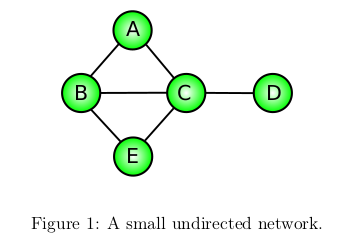
\includegraphics{../assets/fig.png}
\caption{alt text}
\end{figure}

    \subsubsection{a) Your first task is to compute/reason without a
computer the first 4 centrality measures of the above list for the
network shown in Fig.
1}\label{a-your-first-task-is-to-computereason-without-a-computer-the-first-4-centrality-measures-of-the-above-list-for-the-network-shown-in-fig.-1}

the 4 centrality measures: 1. degree \(k(i)\): Number of neighbors of
node \(i\) 2. betweenness centrality \(bc(i)\): \textbf{Number of
shortest paths between other nodes of the network that pass through node
i} 3. closeness centrality \(C(i)\): Inverse of the average shortest
path distance to all other nodes than i: 4. k-shell \(k_s(i)\):
\textbf{Node i belongs to the k-shell, if it belongs to the k-core of
the network but does not belong to the k + 1-core.}

    \begin{enumerate}
\def\labelenumi{\arabic{enumi}.}
\tightlist
\item
  degree \(k(i)\): Number of neighbors of node \(i\) 
\end{enumerate}

\begin{longtable}[]{@{}lll@{}}
\toprule
Node & Degree \(k(i)\)\tabularnewline
\midrule
\endhead
A & 2\tabularnewline
B & 3\tabularnewline
C & 4\tabularnewline
D & 1\tabularnewline
E & 2\tabularnewline
\bottomrule
\end{longtable}

    \begin{enumerate}
\def\labelenumi{\arabic{enumi}.}
\setcounter{enumi}{1}
\tightlist
\item
  betweenness centrality \(bc(i)\): \textbf{Number of shortest paths
  between other nodes of the network that pass through node i} Formally,
  if \(\sigma_{st}\) is the number of shortest paths from s to t and
  \(\sigma_{sit}\) the number of such paths that contain i, then
  \[bc(i) = \frac{1}{(N-2)(N-1)} \sum_{s \neq i} \sum_{t \neq i} \frac{\sigma_{sit}}{\sigma_{st}}\]
  where N = 5
  \[bc(i) = \frac{1}{12} \sum_{s \neq i} \sum_{t \neq i} \frac{\sigma_{sit}}{\sigma_{st}}\]
\end{enumerate}

node A, D, E does not lie on any shortest path (which does not start or
end at itself)

node B lies on the shortest path \(A \rightarrow B \rightarrow E\)

node C lies on the following shortest paths (7): -
\(A \rightarrow C \rightarrow E\) - \(A \rightarrow C \rightarrow D\) -
\(B \rightarrow C \rightarrow D\) - \(D \rightarrow C \rightarrow A\) -
\(D \rightarrow C \rightarrow B\) - \(D \rightarrow C \rightarrow E\) -
\(E \rightarrow C \rightarrow A\) - \(E \rightarrow C \rightarrow D\)

\begin{longtable}[]{@{}lll@{}}
\toprule
Node & betweenness centrality\tabularnewline
\midrule
\endhead
A & 0\tabularnewline
B & 1/12\tabularnewline
C & 7/12\tabularnewline
D & 0\tabularnewline
E & 0\tabularnewline
\bottomrule
\end{longtable}

    \begin{enumerate}
\def\labelenumi{\arabic{enumi}.}
\setcounter{enumi}{2}
\tightlist
\item
  closeness centrality \(C(i)\): Inverse of the average shortest path
  distance to all other nodes than i:
  \[C(i) = \frac{N-1}{\sum_{v \neq i} d(i, v)}\], N=5
\end{enumerate}

\begin{longtable}[]{@{}lll@{}}
\toprule
Node & sum of shortest path & closeness centrality
\(C(i)\)\tabularnewline
\midrule
\endhead
A & 6 & 2/3\tabularnewline
B & 5 & 4/5\tabularnewline
C & 4 & 1\tabularnewline
D & 7 & 4/7\tabularnewline
E & 6 & 2/3\tabularnewline
\bottomrule
\end{longtable}

    \begin{enumerate}
\def\labelenumi{\arabic{enumi}.}
\setcounter{enumi}{3}
\tightlist
\item
  k-shell \(k_s(i)\): \textbf{Node i belongs to the k-shell, if it
  belongs to the k-core of the network but does not belong to the k +
  1-core.}
\end{enumerate}

The k-core is the maximal subnetwork (i.e. the largest possible subset
of the network's nodes, and the links between them) where all nodes have
at least degree k.

In other words, the 1-core is formed by removing nodes of degree 0
(isolated nodes) from the network, the 2-core is formed by removing
nodes of degree 1 and iteratively removing the nodes that become degree
1 or 0 because of the removal, and so on.

The 1-shell is then the set of nodes that was removed from the 1-core to
obtain the 2-core.

\begin{longtable}[]{@{}ll@{}}
\toprule
i-core & set of nodes\tabularnewline
\midrule
\endhead
1-core & \{A,B,C,D,E\}\tabularnewline
2-core & \{A,B,C,E\}\tabularnewline
3-core & \{\}\tabularnewline
\bottomrule
\end{longtable}

    \subsubsection{b) Use NetworkX to compute all five centrality measures
for the
networks}\label{b-use-networkx-to-compute-all-five-centrality-measures-for-the-networks}

shown in Fig 2

\begin{figure}
\centering
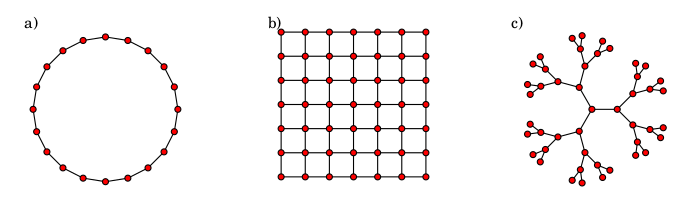
\includegraphics{../assets/fig2.png}
\caption{alt text}
\end{figure}

Figure 2: The model networks. a) A simple ring lattice with N = 20. b) A
simple 2D-lattice with k = 4, L = 7, (N = 49). c) A Cayley tree with k =
3, and l = 4

\textbf{Visualize} - betweenness, - closeness, - k-shell, - eigenvector
centrality

as a function of degree in a scatter plot for each of the networks.

For easier visual comparison of the measures, you should normalize the
k-shell values by dividing them by the maximal k-shell value.

\subsubsection{c) To highlight the differences between the centrality
measures, plot five visualizations for all the networks studied in
b)}\label{c-to-highlight-the-differences-between-the-centrality-measures-plot-five-visualizations-for-all-the-networks-studied-in-b}

(the ring lattice, the 2D-lattice, the Cayley tree and the Karate club
network), each time using one of the centrality mea- sures to define the
colors of the network nodes.

    \begin{Verbatim}[commandchars=\\\{\}]
{\color{incolor}In [{\color{incolor}6}]:} \PY{k+kn}{import} \PY{n+nn}{os}
        \PY{k}{if} \PY{o+ow}{not} \PY{n}{os}\PY{o}{.}\PY{n}{path}\PY{o}{.}\PY{n}{isdir}\PY{p}{(}\PY{l+s+s2}{\PYZdq{}}\PY{l+s+s2}{image\PYZus{}1}\PY{l+s+s2}{\PYZdq{}}\PY{p}{)}\PY{p}{:}
            \PY{n}{os}\PY{o}{.}\PY{n}{makedirs}\PY{p}{(}\PY{l+s+s2}{\PYZdq{}}\PY{l+s+s2}{image\PYZus{}1}\PY{l+s+s2}{\PYZdq{}}\PY{p}{)}
\end{Verbatim}


    \begin{Verbatim}[commandchars=\\\{\}]
{\color{incolor}In [{\color{incolor}1}]:} \PY{k+kn}{import} \PY{n+nn}{networkx} \PY{k}{as} \PY{n+nn}{nx}
        \PY{k+kn}{import} \PY{n+nn}{matplotlib}\PY{n+nn}{.}\PY{n+nn}{pyplot} \PY{k}{as} \PY{n+nn}{plt}
        \PY{k+kn}{import} \PY{n+nn}{numpy} \PY{k}{as} \PY{n+nn}{np}
        
        \PY{k+kn}{from} \PY{n+nn}{centrality\PYZus{}measures\PYZus{}for\PYZus{}undirected\PYZus{}networks} \PY{k}{import} \PY{n}{create\PYZus{}scatter}
        \PY{k+kn}{from} \PY{n+nn}{centrality\PYZus{}measures\PYZus{}for\PYZus{}undirected\PYZus{}networks} \PY{k}{import} \PY{n}{visualize\PYZus{}on\PYZus{}network}
        \PY{k+kn}{from} \PY{n+nn}{centrality\PYZus{}measures\PYZus{}for\PYZus{}undirected\PYZus{}networks} \PY{k}{import} \PY{n}{get\PYZus{}centrality\PYZus{}measures}
        
        \PY{o}{\PYZpc{}}\PY{k}{matplotlib} inline
\end{Verbatim}


    \begin{Verbatim}[commandchars=\\\{\}]
{\color{incolor}In [{\color{incolor}7}]:} \PY{n}{network\PYZus{}paths} \PY{o}{=} \PY{p}{[}\PY{l+s+s1}{\PYZsq{}}\PY{l+s+s1}{.data/small\PYZus{}ring.edg}\PY{l+s+s1}{\PYZsq{}}\PY{p}{,}
                         \PY{l+s+s1}{\PYZsq{}}\PY{l+s+s1}{.data/larger\PYZus{}lattice.edg}\PY{l+s+s1}{\PYZsq{}}\PY{p}{,}
                         \PY{l+s+s1}{\PYZsq{}}\PY{l+s+s1}{.data/small\PYZus{}cayley\PYZus{}tree.edg}\PY{l+s+s1}{\PYZsq{}}\PY{p}{,}
                         \PY{l+s+s1}{\PYZsq{}}\PY{l+s+s1}{.data/karate\PYZus{}club\PYZus{}network\PYZus{}edge\PYZus{}file.edg}\PY{l+s+s1}{\PYZsq{}}\PY{p}{]}
        \PY{n}{coords\PYZus{}paths} \PY{o}{=} \PY{p}{[}\PY{l+s+s1}{\PYZsq{}}\PY{l+s+s1}{.data/small\PYZus{}ring\PYZus{}coords.pkl}\PY{l+s+s1}{\PYZsq{}}\PY{p}{,}
                        \PY{l+s+s1}{\PYZsq{}}\PY{l+s+s1}{.data/larger\PYZus{}lattice\PYZus{}coords.pkl}\PY{l+s+s1}{\PYZsq{}}\PY{p}{,}
                        \PY{l+s+s1}{\PYZsq{}}\PY{l+s+s1}{.data/small\PYZus{}cayley\PYZus{}tree\PYZus{}coords.pkl}\PY{l+s+s1}{\PYZsq{}}\PY{p}{,}
                        \PY{l+s+s1}{\PYZsq{}}\PY{l+s+s1}{.data/karate\PYZus{}club\PYZus{}coords.pkl}\PY{l+s+s1}{\PYZsq{}}\PY{p}{]}
        \PY{n}{network\PYZus{}names} \PY{o}{=} \PY{p}{[}\PY{l+s+s1}{\PYZsq{}}\PY{l+s+s1}{ring}\PY{l+s+s1}{\PYZsq{}}\PY{p}{,} \PY{l+s+s1}{\PYZsq{}}\PY{l+s+s1}{lattice}\PY{l+s+s1}{\PYZsq{}}\PY{p}{,} \PY{l+s+s1}{\PYZsq{}}\PY{l+s+s1}{cayley\PYZus{}tree}\PY{l+s+s1}{\PYZsq{}}\PY{p}{,} \PY{l+s+s1}{\PYZsq{}}\PY{l+s+s1}{karate}\PY{l+s+s1}{\PYZsq{}}\PY{p}{]}
        
        \PY{n}{x\PYZus{}label} \PY{o}{=} \PY{l+s+s1}{\PYZsq{}}\PY{l+s+s1}{Degree k}\PY{l+s+s1}{\PYZsq{}}
        \PY{n}{y\PYZus{}label} \PY{o}{=} \PY{l+s+s1}{\PYZsq{}}\PY{l+s+s1}{Centrality measure}\PY{l+s+s1}{\PYZsq{}}
        \PY{n}{labels} \PY{o}{=} \PY{p}{[}\PY{l+s+s1}{\PYZsq{}}\PY{l+s+s1}{betweenness centrality}\PY{l+s+s1}{\PYZsq{}}\PY{p}{,} \PY{l+s+s1}{\PYZsq{}}\PY{l+s+s1}{closeness centrality}\PY{l+s+s1}{\PYZsq{}}\PY{p}{,}
                  \PY{l+s+s1}{\PYZsq{}}\PY{l+s+s1}{eigenvector centrality}\PY{l+s+s1}{\PYZsq{}}\PY{p}{,} \PY{l+s+s1}{\PYZsq{}}\PY{l+s+s1}{normalized k\PYZhy{}shell}\PY{l+s+s1}{\PYZsq{}}\PY{p}{]}
        \PY{n}{markers} \PY{o}{=} \PY{p}{[}\PY{l+s+s1}{\PYZsq{}}\PY{l+s+s1}{.}\PY{l+s+s1}{\PYZsq{}}\PY{p}{,} \PY{l+s+s1}{\PYZsq{}}\PY{l+s+s1}{x}\PY{l+s+s1}{\PYZsq{}}\PY{p}{,} \PY{l+s+s1}{\PYZsq{}}\PY{l+s+s1}{+}\PY{l+s+s1}{\PYZsq{}}\PY{p}{,} \PY{l+s+s1}{\PYZsq{}}\PY{l+s+s1}{o}\PY{l+s+s1}{\PYZsq{}}\PY{p}{]}
        \PY{n}{scatter\PYZus{}base\PYZus{}path} \PY{o}{=} \PY{l+s+s1}{\PYZsq{}}\PY{l+s+s1}{./centrality\PYZus{}measures\PYZus{}scatter}\PY{l+s+s1}{\PYZsq{}}
        \PY{n}{titles} \PY{o}{=} \PY{p}{[}\PY{l+s+s1}{\PYZsq{}}\PY{l+s+s1}{Degree \PYZdl{}k\PYZdl{}}\PY{l+s+s1}{\PYZsq{}}\PY{p}{,} \PY{l+s+s1}{\PYZsq{}}\PY{l+s+s1}{Betweenness centrality}\PY{l+s+s1}{\PYZsq{}}\PY{p}{,}
                  \PY{l+s+s1}{\PYZsq{}}\PY{l+s+s1}{Closeness centrality}\PY{l+s+s1}{\PYZsq{}}\PY{p}{,} \PY{l+s+s1}{\PYZsq{}}\PY{l+s+s1}{Eigenvector centrality}\PY{l+s+s1}{\PYZsq{}}\PY{p}{,} \PY{l+s+s1}{\PYZsq{}}\PY{l+s+s1}{\PYZdl{}k\PYZdl{}\PYZhy{}shell}\PY{l+s+s1}{\PYZsq{}}\PY{p}{]}
        \PY{n}{network\PYZus{}base\PYZus{}path} \PY{o}{=} \PY{l+s+s1}{\PYZsq{}}\PY{l+s+s1}{./network\PYZus{}figures}\PY{l+s+s1}{\PYZsq{}}
        
        \PY{n}{fig\PYZus{}index} \PY{o}{=} \PY{l+m+mi}{0}
        \PY{n}{tol} \PY{o}{=} \PY{l+m+mi}{10}\PY{o}{*}\PY{o}{*}\PY{o}{\PYZhy{}}\PY{l+m+mi}{1} \PY{c+c1}{\PYZsh{} tolerance parameter for calculating eigenvector centrality}
        
        \PY{c+c1}{\PYZsh{} Loop through all networks}
        \PY{n}{data} \PY{o}{=} \PY{n+nb}{zip}\PY{p}{(}\PY{n}{network\PYZus{}paths}\PY{p}{,} \PY{n}{network\PYZus{}names}\PY{p}{,} \PY{n}{coords\PYZus{}paths}\PY{p}{)}
        \PY{k}{for} \PY{p}{(}\PY{n}{network\PYZus{}path}\PY{p}{,} \PY{n}{network\PYZus{}name}\PY{p}{,} \PY{n}{coords\PYZus{}path}\PY{p}{)} \PY{o+ow}{in} \PY{n}{data}\PY{p}{:}
            \PY{k}{if} \PY{n}{network\PYZus{}name} \PY{o}{==} \PY{l+s+s1}{\PYZsq{}}\PY{l+s+s1}{karate}\PY{l+s+s1}{\PYZsq{}}\PY{p}{:}
                \PY{n}{network} \PY{o}{=} \PY{n}{nx}\PY{o}{.}\PY{n}{read\PYZus{}weighted\PYZus{}edgelist}\PY{p}{(}\PY{n}{network\PYZus{}path}\PY{p}{)}
        
            \PY{k}{else}\PY{p}{:}
                \PY{n}{network} \PY{o}{=} \PY{n}{nx}\PY{o}{.}\PY{n}{read\PYZus{}edgelist}\PY{p}{(}\PY{n}{network\PYZus{}path}\PY{p}{)}
                
            \PY{c+c1}{\PYZsh{} Calculating centrality measures}
            \PY{n}{centrality\PYZus{}measures} \PY{o}{=} \PY{n}{get\PYZus{}centrality\PYZus{}measures}\PY{p}{(}\PY{n}{network}\PY{p}{,} \PY{n}{tol}\PY{p}{)}
            \PY{p}{[}\PY{n}{degree}\PY{p}{,} \PY{n}{betweenness}\PY{p}{,} \PY{n}{closeness}\PY{p}{,} \PY{n}{eigenvector\PYZus{}centrality}\PY{p}{,} \PY{n}{kshell}\PY{p}{]} \PY{o}{=} \PY{n}{centrality\PYZus{}measures}
            \PY{n}{kshell\PYZus{}normalized} \PY{o}{=} \PY{n}{kshell}\PY{o}{/}\PY{n+nb}{float}\PY{p}{(}\PY{n}{np}\PY{o}{.}\PY{n}{max}\PY{p}{(}\PY{n}{kshell}\PY{p}{)}\PY{p}{)} \PY{c+c1}{\PYZsh{} normalization}
            \PY{c+c1}{\PYZsh{} Scatter plot}
            \PY{n}{y\PYZus{}values} \PY{o}{=} \PY{p}{[}\PY{n}{betweenness}\PY{p}{,} \PY{n}{closeness}\PY{p}{,} \PY{n}{eigenvector\PYZus{}centrality}\PY{p}{,} \PY{n}{kshell\PYZus{}normalized}\PY{p}{]}
            \PY{n}{scatter\PYZus{}path} \PY{o}{=} \PY{n}{scatter\PYZus{}base\PYZus{}path} \PY{o}{+} \PY{l+s+s1}{\PYZsq{}}\PY{l+s+s1}{\PYZus{}}\PY{l+s+s1}{\PYZsq{}} \PY{o}{+} \PY{n}{network\PYZus{}name} \PY{o}{+} \PY{l+s+s1}{\PYZsq{}}\PY{l+s+s1}{.png}\PY{l+s+s1}{\PYZsq{}}
        
            \PY{n}{fig} \PY{o}{=} \PY{n}{create\PYZus{}scatter}\PY{p}{(}\PY{n}{degree}\PY{p}{,} \PY{n}{y\PYZus{}values}\PY{p}{,} \PY{n}{x\PYZus{}label}\PY{p}{,} \PY{n}{y\PYZus{}label}\PY{p}{,} \PY{n}{labels}\PY{p}{,} \PY{n}{markers}\PY{p}{)}
            \PY{n}{fig}\PY{o}{.}\PY{n}{suptitle}\PY{p}{(}\PY{n}{network\PYZus{}name}\PY{p}{,} \PY{n}{size}\PY{o}{=}\PY{l+m+mi}{20}\PY{p}{)}
            \PY{n}{plt}\PY{o}{.}\PY{n}{show}\PY{p}{(}\PY{p}{)}
            \PY{n}{fig}\PY{o}{.}\PY{n}{savefig}\PY{p}{(}\PY{l+s+s2}{\PYZdq{}}\PY{l+s+s2}{image\PYZus{}1/}\PY{l+s+s2}{\PYZdq{}} \PY{o}{+} \PY{n}{scatter\PYZus{}path}\PY{p}{)}
        
        
            \PY{c+c1}{\PYZsh{} Network figures}
            \PY{n}{network\PYZus{}figure\PYZus{}path} \PY{o}{=} \PY{n}{network\PYZus{}base\PYZus{}path} \PY{o}{+} \PY{l+s+s1}{\PYZsq{}}\PY{l+s+s1}{\PYZus{}}\PY{l+s+s1}{\PYZsq{}} \PY{o}{+} \PY{n}{network\PYZus{}name} \PY{o}{+} \PY{l+s+s1}{\PYZsq{}}\PY{l+s+s1}{.png}\PY{l+s+s1}{\PYZsq{}}
            \PY{n}{all\PYZus{}cvalues} \PY{o}{=} \PY{p}{[}\PY{n}{degree}\PY{p}{,} \PY{n}{betweenness}\PY{p}{,} \PY{n}{closeness}\PY{p}{,} \PY{n}{eigenvector\PYZus{}centrality}\PY{p}{,} \PY{n}{kshell}\PY{p}{]}
            \PY{n}{fig}\PY{o}{=}\PY{n}{visualize\PYZus{}on\PYZus{}network}\PY{p}{(}\PY{n}{network}\PY{p}{,} \PY{n}{all\PYZus{}cvalues}\PY{p}{,}
                                     \PY{n}{coords\PYZus{}path}\PY{p}{,} \PY{n}{titles}\PY{p}{)}
            
            \PY{n}{fig}\PY{o}{.}\PY{n}{savefig}\PY{p}{(}\PY{l+s+s2}{\PYZdq{}}\PY{l+s+s2}{image\PYZus{}1/}\PY{l+s+s2}{\PYZdq{}} \PY{o}{+} \PY{n}{network\PYZus{}figure\PYZus{}path}\PY{p}{)}
\end{Verbatim}


    \begin{center}
    \adjustimage{max size={0.9\linewidth}{0.9\paperheight}}{output_11_0.png}
    \end{center}
    { \hspace*{\fill} \\}
    
    \begin{center}
    \adjustimage{max size={0.9\linewidth}{0.9\paperheight}}{output_11_1.png}
    \end{center}
    { \hspace*{\fill} \\}
    
    \begin{center}
    \adjustimage{max size={0.9\linewidth}{0.9\paperheight}}{output_11_2.png}
    \end{center}
    { \hspace*{\fill} \\}
    
    \begin{center}
    \adjustimage{max size={0.9\linewidth}{0.9\paperheight}}{output_11_3.png}
    \end{center}
    { \hspace*{\fill} \\}
    
    \begin{center}
    \adjustimage{max size={0.9\linewidth}{0.9\paperheight}}{output_11_4.png}
    \end{center}
    { \hspace*{\fill} \\}
    
    \begin{center}
    \adjustimage{max size={0.9\linewidth}{0.9\paperheight}}{output_11_5.png}
    \end{center}
    { \hspace*{\fill} \\}
    
    \begin{center}
    \adjustimage{max size={0.9\linewidth}{0.9\paperheight}}{output_11_6.png}
    \end{center}
    { \hspace*{\fill} \\}
    
    \begin{center}
    \adjustimage{max size={0.9\linewidth}{0.9\paperheight}}{output_11_7.png}
    \end{center}
    { \hspace*{\fill} \\}
    
    \subsubsection{d) Based on the results of a) and b), how do these
centralities differ from each
other?}\label{d-based-on-the-results-of-a-and-b-how-do-these-centralities-differ-from-each-other}

Would you say that some of them do a better or worse job than others in
identifying central nodes? To answer the questions, you can for example
pick some representative nodes and try to explain why different
centrality measures rank these nodes differently regarding its
centrality. In your answer, briefly cover all the networks visualized in
c).

\textbf{Ans}

The \textbf{k-shell centrality} only works on the karate network. It
gives value of how similar two well-connected nodes are.

The \textbf{betweenness centrality} depends on the shortest paths.
\textbf{closeness centrality} is depends on the distance of a node to
other nodes. It is interesting to see that both of these centralities
produce quite similar results as one another, as observed in the
2d-lattice and cayley trees. These two centralities give higher values
to nodes in the centre (which we can deem as more important) and the
further away from the center, the lower the values become

The \textbf{Eigenvector centrality} is depends on node degrees of the
own nodes as well as the neighbours node. This centrality seems to
perform somewhere between the \textbf{degree} centrality and the
\textbf{betweeness/ closeness}

    \section{Degree correlations and
assortativity}\label{degree-correlations-and-assortativity}

In this problem, we consider degree correlations and assortativity of
two real-world networks: - the Zachary karate club network
(\texttt{karate\_club\_network\_edge\_file.edg}) - a snowball-sampled
subgraph of a Facebook friendships network
(\texttt{facebook-wosn-links\_subgraph.edg}).

For both networks, perform the following analyses:

\subsubsection{a) Create a scatter plot of the degrees of pairs of
connected
nodes.}\label{a-create-a-scatter-plot-of-the-degrees-of-pairs-of-connected-nodes.}

That is, take - each connected pair of nodes \((i,j)\), - take their
degrees \(k_i\) and \(k_j\) , - plot the point (\(k_i\) , \(k_j\) ) on
two axes with degrees as their units, and - repeat for all pairs of
connected nodes.

Because the network is undirected, the plot should be symmetrical,
containing points (\(k_i\) , \(k_j\) ) and (\(k_j\) , \(k_i\) ) for all
connected pairs (\(i,j\)).

\subsubsection{b) Produce a heat map 1 of the degrees of all connected
nodes.}\label{b-produce-a-heat-map-1-of-the-degrees-of-all-connected-nodes.}

The heat map uses the same information as you used in a), that is, the
degrees of pairs of connected nodes. However, no points are plotted:
rather, the two degree axes are binned and the number of degree pairs
(\(k_i\) , \(k_j\) ) in each bin is computed. Then, the bin is colored
according to this number (e.g., red = many connected pairs of nodes with
degrees falling in the bin).

\begin{itemize}
\tightlist
\item
  What extra information do you gain by using a he1atmap instead of just
  a scatter plot (if any)? \textbf{Ans} The heat maps offers 1 more
  dimension of data, Frequency/Occurence/Count of that combination of
  pair of node, via color.
\end{itemize}

    \begin{Verbatim}[commandchars=\\\{\}]
{\color{incolor}In [{\color{incolor}8}]:} \PY{k+kn}{from} \PY{n+nn}{degree\PYZus{}correlations\PYZus{}assortativity} \PY{k}{import} \PY{n}{create\PYZus{}scatter}
        \PY{k+kn}{from} \PY{n+nn}{degree\PYZus{}correlations\PYZus{}assortativity} \PY{k}{import} \PY{n}{create\PYZus{}heatmap}
        \PY{k+kn}{from} \PY{n+nn}{degree\PYZus{}correlations\PYZus{}assortativity} \PY{k}{import} \PY{n}{visualize\PYZus{}nearest\PYZus{}neighbor\PYZus{}degree}
        
        \PY{k+kn}{from} \PY{n+nn}{degree\PYZus{}correlations\PYZus{}assortativity} \PY{k}{import} \PY{n}{get\PYZus{}x\PYZus{}and\PYZus{}y\PYZus{}degrees}
        \PY{k+kn}{from} \PY{n+nn}{degree\PYZus{}correlations\PYZus{}assortativity} \PY{k}{import} \PY{n}{assortativity}
        \PY{k+kn}{from} \PY{n+nn}{degree\PYZus{}correlations\PYZus{}assortativity} \PY{k}{import} \PY{n}{get\PYZus{}nearest\PYZus{}neighbor\PYZus{}degree}
        \PY{k+kn}{from} \PY{n+nn}{degree\PYZus{}correlations\PYZus{}assortativity} \PY{k}{import} \PY{n}{get\PYZus{}simple\PYZus{}bin\PYZus{}average}
\end{Verbatim}


    \begin{Verbatim}[commandchars=\\\{\}]
{\color{incolor}In [{\color{incolor}9}]:} \PY{k+kn}{import} \PY{n+nn}{os}
        \PY{k}{if} \PY{o+ow}{not} \PY{n}{os}\PY{o}{.}\PY{n}{path}\PY{o}{.}\PY{n}{isdir}\PY{p}{(}\PY{l+s+s2}{\PYZdq{}}\PY{l+s+s2}{image\PYZus{}2}\PY{l+s+s2}{\PYZdq{}}\PY{p}{)}\PY{p}{:}
            \PY{n}{os}\PY{o}{.}\PY{n}{makedirs}\PY{p}{(}\PY{l+s+s2}{\PYZdq{}}\PY{l+s+s2}{image\PYZus{}2}\PY{l+s+s2}{\PYZdq{}}\PY{p}{)}
\end{Verbatim}


    \begin{Verbatim}[commandchars=\\\{\}]
{\color{incolor}In [{\color{incolor}10}]:} \PY{n}{network\PYZus{}paths} \PY{o}{=} \PY{p}{[}\PY{l+s+s1}{\PYZsq{}}\PY{l+s+s1}{./data/karate\PYZus{}club\PYZus{}network\PYZus{}edge\PYZus{}file.edg}\PY{l+s+s1}{\PYZsq{}}\PY{p}{,}
                          \PY{l+s+s1}{\PYZsq{}}\PY{l+s+s1}{./data/facebook\PYZhy{}wosn\PYZhy{}links\PYZus{}subgraph.edg}\PY{l+s+s1}{\PYZsq{}}\PY{p}{]}
         \PY{n}{network\PYZus{}names} \PY{o}{=} \PY{p}{[}\PY{l+s+s1}{\PYZsq{}}\PY{l+s+s1}{karate}\PY{l+s+s1}{\PYZsq{}}\PY{p}{,} \PY{l+s+s1}{\PYZsq{}}\PY{l+s+s1}{facebook}\PY{l+s+s1}{\PYZsq{}}\PY{p}{]}
         \PY{n}{network\PYZus{}titles} \PY{o}{=} \PY{p}{[}\PY{l+s+s1}{\PYZsq{}}\PY{l+s+s1}{Karate Club Network}\PY{l+s+s1}{\PYZsq{}}\PY{p}{,}
                           \PY{l+s+s1}{\PYZsq{}}\PY{l+s+s1}{Facebook Friendship Network}\PY{l+s+s1}{\PYZsq{}}\PY{p}{]}
         \PY{n}{scatter\PYZus{}figure\PYZus{}base} \PY{o}{=} \PY{l+s+s1}{\PYZsq{}}\PY{l+s+s1}{./image\PYZus{}2/edge\PYZus{}degree\PYZus{}correlation\PYZus{}scatter\PYZus{}}\PY{l+s+s1}{\PYZsq{}}
         \PY{n}{heatmap\PYZus{}figure\PYZus{}base} \PY{o}{=} \PY{l+s+s1}{\PYZsq{}}\PY{l+s+s1}{./image\PYZus{}2/heatmap\PYZus{}}\PY{l+s+s1}{\PYZsq{}}
         \PY{n}{nearest\PYZus{}neighbor\PYZus{}figure\PYZus{}base} \PY{o}{=} \PY{l+s+s1}{\PYZsq{}}\PY{l+s+s1}{./image\PYZus{}2/nearest\PYZus{}}\PY{l+s+s1}{\PYZsq{}}
\end{Verbatim}


    \begin{Verbatim}[commandchars=\\\{\}]
{\color{incolor}In [{\color{incolor}11}]:} \PY{c+c1}{\PYZsh{} Loop through all networks}
         
         \PY{n}{data} \PY{o}{=} \PY{n+nb}{zip}\PY{p}{(}\PY{n}{network\PYZus{}paths}\PY{p}{,} \PY{n}{network\PYZus{}names}\PY{p}{,} \PY{n}{network\PYZus{}titles}\PY{p}{)}
         \PY{k}{for} \PY{n}{network\PYZus{}path}\PY{p}{,} \PY{n}{network\PYZus{}name}\PY{p}{,} \PY{n}{network\PYZus{}title} \PY{o+ow}{in} \PY{n}{data}\PY{p}{:}
             \PY{n}{network} \PY{o}{=} \PY{n}{nx}\PY{o}{.}\PY{n}{read\PYZus{}weighted\PYZus{}edgelist}\PY{p}{(}\PY{n}{network\PYZus{}path}\PY{p}{)}
             \PY{n}{x\PYZus{}degrees}\PY{p}{,} \PY{n}{y\PYZus{}degrees} \PY{o}{=} \PY{n}{get\PYZus{}x\PYZus{}and\PYZus{}y\PYZus{}degrees}\PY{p}{(}\PY{n}{network}\PY{p}{)}
         
             \PY{n}{fig} \PY{o}{=} \PY{n}{create\PYZus{}scatter}\PY{p}{(}\PY{n}{x\PYZus{}degrees}\PY{p}{,} \PY{n}{y\PYZus{}degrees}\PY{p}{,} \PY{n}{network\PYZus{}title}\PY{p}{)}
             \PY{n}{fig}\PY{o}{.}\PY{n}{savefig}\PY{p}{(}\PY{n}{scatter\PYZus{}figure\PYZus{}base}\PY{o}{+}\PY{n}{network\PYZus{}name}\PY{o}{+}\PY{l+s+s1}{\PYZsq{}}\PY{l+s+s1}{.pdf}\PY{l+s+s1}{\PYZsq{}}\PY{p}{)}
         
             \PY{n}{fig} \PY{o}{=} \PY{n}{create\PYZus{}heatmap}\PY{p}{(}\PY{n}{x\PYZus{}degrees}\PY{p}{,} \PY{n}{y\PYZus{}degrees}\PY{p}{,} \PY{n}{network\PYZus{}title}\PY{p}{)}
             \PY{n}{fig}\PY{o}{.}\PY{n}{savefig}\PY{p}{(}\PY{n}{heatmap\PYZus{}figure\PYZus{}base}\PY{o}{+}\PY{n}{network\PYZus{}name}\PY{o}{+}\PY{l+s+s1}{\PYZsq{}}\PY{l+s+s1}{.pdf}\PY{l+s+s1}{\PYZsq{}}\PY{p}{)}
         
             \PY{c+c1}{\PYZsh{} assortativities}
             \PY{n}{assortativity\PYZus{}own} \PY{o}{=} \PY{n}{assortativity}\PY{p}{(}\PY{n}{x\PYZus{}degrees}\PY{p}{,} \PY{n}{y\PYZus{}degrees}\PY{p}{)}
             \PY{n}{assortativity\PYZus{}nx} \PY{o}{=} \PY{n}{nx}\PY{o}{.}\PY{n}{degree\PYZus{}assortativity\PYZus{}coefficient}\PY{p}{(}\PY{n}{network}\PY{p}{)}
             \PY{n+nb}{print}\PY{p}{(}\PY{l+s+s2}{\PYZdq{}}\PY{l+s+s2}{Own assortativity for }\PY{l+s+s2}{\PYZdq{}} \PY{o}{+} \PY{n}{network\PYZus{}title} \PY{o}{+} \PY{l+s+s2}{\PYZdq{}}\PY{l+s+s2}{: }\PY{l+s+s2}{\PYZdq{}} \PY{o}{+}
                   \PY{n+nb}{str}\PY{p}{(}\PY{n}{assortativity\PYZus{}own}\PY{p}{)}\PY{p}{)}
             \PY{n+nb}{print}\PY{p}{(}\PY{l+s+s2}{\PYZdq{}}\PY{l+s+s2}{NetworkX assortativity for }\PY{l+s+s2}{\PYZdq{}} \PY{o}{+} \PY{n}{network\PYZus{}title} \PY{o}{+} \PY{l+s+s2}{\PYZdq{}}\PY{l+s+s2}{: }\PY{l+s+s2}{\PYZdq{}} \PY{o}{+}
                   \PY{n+nb}{str}\PY{p}{(}\PY{n}{assortativity\PYZus{}nx}\PY{p}{)}\PY{p}{)}
         
             \PY{c+c1}{\PYZsh{} nearest neighbor degrees}
             \PY{n}{degrees}\PY{p}{,} \PY{n}{nearest\PYZus{}neighbor\PYZus{}degrees} \PY{o}{=} \PY{n}{get\PYZus{}nearest\PYZus{}neighbor\PYZus{}degree}\PY{p}{(}\PY{n}{network}\PY{p}{)}
             \PY{n}{unique\PYZus{}degrees}\PY{p}{,} \PY{n}{mean\PYZus{}nearest\PYZus{}neighbor\PYZus{}degrees} \PY{o}{=} \PY{n}{get\PYZus{}simple\PYZus{}bin\PYZus{}average}\PY{p}{(}
                 \PY{n}{degrees}\PY{p}{,}
                 \PY{n}{nearest\PYZus{}neighbor\PYZus{}degrees}
             \PY{p}{)}
             \PY{n}{fig} \PY{o}{=} \PY{n}{visualize\PYZus{}nearest\PYZus{}neighbor\PYZus{}degree}\PY{p}{(}\PY{n}{degrees}\PY{p}{,}
                                                     \PY{n}{nearest\PYZus{}neighbor\PYZus{}degrees}\PY{p}{,}
                                                     \PY{n}{unique\PYZus{}degrees}\PY{p}{,}
                                                     \PY{n}{mean\PYZus{}nearest\PYZus{}neighbor\PYZus{}degrees}\PY{p}{,}
                                                     \PY{n}{network\PYZus{}title}\PY{p}{)}
             \PY{n}{fig}\PY{o}{.}\PY{n}{savefig}\PY{p}{(}\PY{n}{nearest\PYZus{}neighbor\PYZus{}figure\PYZus{}base} \PY{o}{+} \PY{n}{network\PYZus{}name} \PY{o}{+} \PY{l+s+s1}{\PYZsq{}}\PY{l+s+s1}{.pdf}\PY{l+s+s1}{\PYZsq{}}\PY{p}{)}
             \PY{n}{plt}\PY{o}{.}\PY{n}{show}\PY{p}{(}\PY{p}{)}
\end{Verbatim}


    \begin{Verbatim}[commandchars=\\\{\}]
Own assortativity for Karate Club Network: -0.47136675756640545
NetworkX assortativity for Karate Club Network: -0.47561309768461457

    \end{Verbatim}

    \begin{Verbatim}[commandchars=\\\{\}]
/home/adam/Desktop/work/complex-networks/week6/code/degree\_correlations\_assortativity.py:224: RuntimeWarning: invalid value encountered in double\_scalars
  bin\_average[i] = bin\_average[i]/denominator

    \end{Verbatim}

    \begin{center}
    \adjustimage{max size={0.9\linewidth}{0.9\paperheight}}{output_17_2.png}
    \end{center}
    { \hspace*{\fill} \\}
    
    \begin{center}
    \adjustimage{max size={0.9\linewidth}{0.9\paperheight}}{output_17_3.png}
    \end{center}
    { \hspace*{\fill} \\}
    
    \begin{center}
    \adjustimage{max size={0.9\linewidth}{0.9\paperheight}}{output_17_4.png}
    \end{center}
    { \hspace*{\fill} \\}
    
    \begin{Verbatim}[commandchars=\\\{\}]
Own assortativity for Facebook Friendship Network: 0.05596269693739395
NetworkX assortativity for Facebook Friendship Network: 0.05598478476593048

    \end{Verbatim}

    \begin{center}
    \adjustimage{max size={0.9\linewidth}{0.9\paperheight}}{output_17_6.png}
    \end{center}
    { \hspace*{\fill} \\}
    
    \begin{center}
    \adjustimage{max size={0.9\linewidth}{0.9\paperheight}}{output_17_7.png}
    \end{center}
    { \hspace*{\fill} \\}
    
    \begin{center}
    \adjustimage{max size={0.9\linewidth}{0.9\paperheight}}{output_17_8.png}
    \end{center}
    { \hspace*{\fill} \\}
    
    \subsubsection{c)}\label{c}

The assortativity coefficient is defined as the Pearson correlation
coefficient of the degrees of pairs of connected nodes. Calculate the
assortativity coefficient of the network using
\texttt{scipy.stats.pearsonr} and compare your result with the output of
\texttt{NetworkX} function \texttt{degree\_assortativity\_coefficient}.
As mentioned in the lecture, social networks typically are assortative.

\textbf{Ans.} Karate Club Network - Own assortativity for Karate Club
Network: -0.47136675756640545 - NetworkX assortativity for Karate Club
Network: -0.47561309768461457

Facebook Friendship Network - Own assortativity for Facebook Friendship
Network: 0.05596269693739395 - NetworkX assortativity for Facebook
Friendship Network: 0.05598478476593048

\subsubsection{Does this hold for these two social networks? What could
explain this
result?}\label{does-this-hold-for-these-two-social-networks-what-could-explain-this-result}

\textbf{Ans.} - Karate Club is not assortative (-0.47 Negative) due to
conflicts in the club, forming 2 clusters, leading to the split of the
club - The Facebook Friendship network is assortative (0.055 Positive),
as it is a social network.

    \subsubsection{\texorpdfstring{d) For each node, compute the average
nearest neighbour degree \(k_{nn}\)
and}{d) For each node, compute the average nearest neighbour degree k\_\{nn\} and}}\label{d-for-each-node-compute-the-average-nearest-neighbour-degree-k_nn-and}

make a scatter plot of \(k _{nn}\) as a function of \(k\). In the same
plot, plot also the curve of \(\langle k_{nn} \rangle (k)\) as a
function of \(k\), i.e. the averaged \(k_{nn}\) for each \(k\). Comment
the result from the viewpoint of assortativity.

\textbf{Ans.} Particularly for a larger network such as the facebook
friendship network, with a larger degree, we can be more confident that
it's neighbours also has a large degree.

This means that high-degree nodes link to other high-degree nodes.

We can explain this through homophily, where people tend to form social
ties to others like them.

    \section{Bipartite networks}\label{bipartite-networks}

Consider the bipartite network of actors and movies shown in Figure 3.

\begin{figure}
\centering
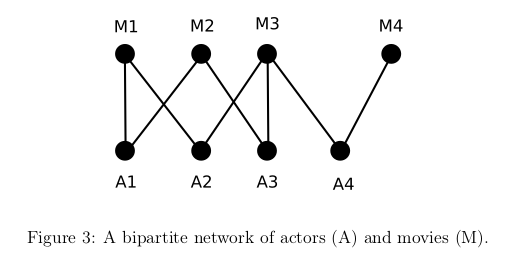
\includegraphics{../assets/fig3.png}
\caption{alt text}
\end{figure}

\subsubsection{a) Construct the two unipartite projections of the
network -- the network of actors and the network of
movies.}\label{a-construct-the-two-unipartite-projections-of-the-network-the-network-of-actors-and-the-network-of-movies.}

In the former, actors are linked if they have acted together in at least
one movie, and in the latter, movies are linked if there is at least one
common actor.

    \begin{Verbatim}[commandchars=\\\{\}]
{\color{incolor}In [{\color{incolor}12}]:} \PY{k+kn}{from} \PY{n+nn}{networkx}\PY{n+nn}{.}\PY{n+nn}{algorithms} \PY{k}{import} \PY{n}{bipartite}
         
         \PY{n}{fig} \PY{o}{=} \PY{n}{nx}\PY{o}{.}\PY{n}{Graph}\PY{p}{(}\PY{p}{)}
         
         \PY{n}{fig}\PY{o}{.}\PY{n}{add\PYZus{}nodes\PYZus{}from}\PY{p}{(}\PY{p}{[}\PY{l+s+s1}{\PYZsq{}}\PY{l+s+s1}{M1}\PY{l+s+s1}{\PYZsq{}}\PY{p}{,} \PY{l+s+s1}{\PYZsq{}}\PY{l+s+s1}{M2}\PY{l+s+s1}{\PYZsq{}}\PY{p}{,} \PY{l+s+s1}{\PYZsq{}}\PY{l+s+s1}{M3}\PY{l+s+s1}{\PYZsq{}}\PY{p}{,} \PY{l+s+s1}{\PYZsq{}}\PY{l+s+s1}{M4}\PY{l+s+s1}{\PYZsq{}}\PY{p}{]}\PY{p}{,} \PY{n}{bipartite}\PY{o}{=}\PY{l+m+mi}{0}\PY{p}{)}
         \PY{n}{fig}\PY{o}{.}\PY{n}{add\PYZus{}nodes\PYZus{}from}\PY{p}{(}\PY{p}{[}\PY{l+s+s1}{\PYZsq{}}\PY{l+s+s1}{A1}\PY{l+s+s1}{\PYZsq{}}\PY{p}{,} \PY{l+s+s1}{\PYZsq{}}\PY{l+s+s1}{A2}\PY{l+s+s1}{\PYZsq{}}\PY{p}{,} \PY{l+s+s1}{\PYZsq{}}\PY{l+s+s1}{A3}\PY{l+s+s1}{\PYZsq{}}\PY{p}{,} \PY{l+s+s1}{\PYZsq{}}\PY{l+s+s1}{A4}\PY{l+s+s1}{\PYZsq{}}\PY{p}{]}\PY{p}{,} \PY{n}{bipartite}\PY{o}{=}\PY{l+m+mi}{1}\PY{p}{)}
         
         \PY{n}{fig}\PY{o}{.}\PY{n}{add\PYZus{}edges\PYZus{}from}\PY{p}{(}\PY{p}{[}\PY{p}{(}\PY{l+s+s1}{\PYZsq{}}\PY{l+s+s1}{M1}\PY{l+s+s1}{\PYZsq{}}\PY{p}{,} \PY{l+s+s1}{\PYZsq{}}\PY{l+s+s1}{A1}\PY{l+s+s1}{\PYZsq{}}\PY{p}{)}\PY{p}{,} \PY{p}{(}\PY{l+s+s1}{\PYZsq{}}\PY{l+s+s1}{M1}\PY{l+s+s1}{\PYZsq{}}\PY{p}{,} \PY{l+s+s1}{\PYZsq{}}\PY{l+s+s1}{A2}\PY{l+s+s1}{\PYZsq{}}\PY{p}{)}\PY{p}{,}
                             \PY{p}{(}\PY{l+s+s1}{\PYZsq{}}\PY{l+s+s1}{M2}\PY{l+s+s1}{\PYZsq{}}\PY{p}{,} \PY{l+s+s1}{\PYZsq{}}\PY{l+s+s1}{A1}\PY{l+s+s1}{\PYZsq{}}\PY{p}{)}\PY{p}{,} \PY{p}{(}\PY{l+s+s1}{\PYZsq{}}\PY{l+s+s1}{M2}\PY{l+s+s1}{\PYZsq{}}\PY{p}{,} \PY{l+s+s1}{\PYZsq{}}\PY{l+s+s1}{A3}\PY{l+s+s1}{\PYZsq{}}\PY{p}{)}\PY{p}{,}                    
                             \PY{p}{(}\PY{l+s+s1}{\PYZsq{}}\PY{l+s+s1}{M3}\PY{l+s+s1}{\PYZsq{}}\PY{p}{,} \PY{l+s+s1}{\PYZsq{}}\PY{l+s+s1}{A2}\PY{l+s+s1}{\PYZsq{}}\PY{p}{)}\PY{p}{,} \PY{p}{(}\PY{l+s+s1}{\PYZsq{}}\PY{l+s+s1}{M3}\PY{l+s+s1}{\PYZsq{}}\PY{p}{,} \PY{l+s+s1}{\PYZsq{}}\PY{l+s+s1}{A3}\PY{l+s+s1}{\PYZsq{}}\PY{p}{)}\PY{p}{,}  
                             \PY{p}{(}\PY{l+s+s1}{\PYZsq{}}\PY{l+s+s1}{M3}\PY{l+s+s1}{\PYZsq{}}\PY{p}{,} \PY{l+s+s1}{\PYZsq{}}\PY{l+s+s1}{A4}\PY{l+s+s1}{\PYZsq{}}\PY{p}{)}\PY{p}{,} \PY{p}{(}\PY{l+s+s1}{\PYZsq{}}\PY{l+s+s1}{M4}\PY{l+s+s1}{\PYZsq{}}\PY{p}{,} \PY{l+s+s1}{\PYZsq{}}\PY{l+s+s1}{A4}\PY{l+s+s1}{\PYZsq{}}\PY{p}{)}\PY{p}{]}\PY{p}{)}
         
         \PY{n}{movies}\PY{p}{,} \PY{n}{actors} \PY{o}{=} \PY{n}{bipartite}\PY{o}{.}\PY{n}{sets}\PY{p}{(}\PY{n}{fig}\PY{p}{)}
         
         \PY{n}{plt}\PY{o}{.}\PY{n}{suptitle}\PY{p}{(}\PY{l+s+s2}{\PYZdq{}}\PY{l+s+s2}{Movies}\PY{l+s+s2}{\PYZdq{}}\PY{p}{)}
         \PY{n}{nx}\PY{o}{.}\PY{n}{draw}\PY{p}{(}\PY{n}{bipartite}\PY{o}{.}\PY{n}{projected\PYZus{}graph}\PY{p}{(}\PY{n}{B}\PY{o}{=}\PY{n}{fig}\PY{p}{,} \PY{n}{nodes}\PY{o}{=}\PY{n}{movies}\PY{p}{)}\PY{p}{,} \PY{n}{with\PYZus{}labels}\PY{o}{=}\PY{k+kc}{True}\PY{p}{)}
         \PY{n}{plt}\PY{o}{.}\PY{n}{show}\PY{p}{(}\PY{p}{)}
         
         \PY{n}{plt}\PY{o}{.}\PY{n}{suptitle}\PY{p}{(}\PY{l+s+s2}{\PYZdq{}}\PY{l+s+s2}{Actors}\PY{l+s+s2}{\PYZdq{}}\PY{p}{)}
         \PY{n}{nx}\PY{o}{.}\PY{n}{draw}\PY{p}{(}\PY{n}{bipartite}\PY{o}{.}\PY{n}{projected\PYZus{}graph}\PY{p}{(}\PY{n}{B}\PY{o}{=}\PY{n}{fig}\PY{p}{,} \PY{n}{nodes}\PY{o}{=}\PY{n}{actors}\PY{p}{)}\PY{p}{,} \PY{n}{with\PYZus{}labels}\PY{o}{=}\PY{k+kc}{True}\PY{p}{)}
         \PY{n}{plt}\PY{o}{.}\PY{n}{show}\PY{p}{(}\PY{p}{)}
\end{Verbatim}


    \begin{center}
    \adjustimage{max size={0.9\linewidth}{0.9\paperheight}}{output_21_0.png}
    \end{center}
    { \hspace*{\fill} \\}
    
    \begin{center}
    \adjustimage{max size={0.9\linewidth}{0.9\paperheight}}{output_21_1.png}
    \end{center}
    { \hspace*{\fill} \\}
    
    \subsubsection{b) Show that, in general, it is not possible to uniquely
reconstruct a bipartite network from its two unipartite
projections.}\label{b-show-that-in-general-it-is-not-possible-to-uniquely-reconstruct-a-bipartite-network-from-its-two-unipartite-projections.}

Prove this by providing a counterexample: Take the same 4 actors and 4
movies, and design a different bipartite network that has exactly the
same unipartite projections. That is, connect the actors and movies in
some way that results in the same projections as in a).

    \begin{Verbatim}[commandchars=\\\{\}]
{\color{incolor}In [{\color{incolor}14}]:} \PY{n}{fig2} \PY{o}{=} \PY{n}{nx}\PY{o}{.}\PY{n}{Graph}\PY{p}{(}\PY{p}{)}
         
         \PY{n}{fig2}\PY{o}{.}\PY{n}{add\PYZus{}nodes\PYZus{}from}\PY{p}{(}\PY{p}{[}\PY{l+s+s1}{\PYZsq{}}\PY{l+s+s1}{M1}\PY{l+s+s1}{\PYZsq{}}\PY{p}{,} \PY{l+s+s1}{\PYZsq{}}\PY{l+s+s1}{M2}\PY{l+s+s1}{\PYZsq{}}\PY{p}{,} \PY{l+s+s1}{\PYZsq{}}\PY{l+s+s1}{M3}\PY{l+s+s1}{\PYZsq{}}\PY{p}{,} \PY{l+s+s1}{\PYZsq{}}\PY{l+s+s1}{M4}\PY{l+s+s1}{\PYZsq{}}\PY{p}{]}\PY{p}{,} \PY{n}{bipartite}\PY{o}{=}\PY{l+m+mi}{0}\PY{p}{)}
         \PY{n}{fig2}\PY{o}{.}\PY{n}{add\PYZus{}nodes\PYZus{}from}\PY{p}{(}\PY{p}{[}\PY{l+s+s1}{\PYZsq{}}\PY{l+s+s1}{A1}\PY{l+s+s1}{\PYZsq{}}\PY{p}{,} \PY{l+s+s1}{\PYZsq{}}\PY{l+s+s1}{A2}\PY{l+s+s1}{\PYZsq{}}\PY{p}{,} \PY{l+s+s1}{\PYZsq{}}\PY{l+s+s1}{A3}\PY{l+s+s1}{\PYZsq{}}\PY{p}{,} \PY{l+s+s1}{\PYZsq{}}\PY{l+s+s1}{A4}\PY{l+s+s1}{\PYZsq{}}\PY{p}{]}\PY{p}{,} \PY{n}{bipartite}\PY{o}{=}\PY{l+m+mi}{1}\PY{p}{)}
         
         \PY{n}{fig2}\PY{o}{.}\PY{n}{add\PYZus{}edges\PYZus{}from}\PY{p}{(}\PY{p}{[}\PY{p}{(}\PY{l+s+s1}{\PYZsq{}}\PY{l+s+s1}{M1}\PY{l+s+s1}{\PYZsq{}}\PY{p}{,} \PY{l+s+s1}{\PYZsq{}}\PY{l+s+s1}{A4}\PY{l+s+s1}{\PYZsq{}}\PY{p}{)}\PY{p}{,} \PY{p}{(}\PY{l+s+s1}{\PYZsq{}}\PY{l+s+s1}{M1}\PY{l+s+s1}{\PYZsq{}}\PY{p}{,} \PY{l+s+s1}{\PYZsq{}}\PY{l+s+s1}{A2}\PY{l+s+s1}{\PYZsq{}}\PY{p}{)}\PY{p}{,}
                             \PY{p}{(}\PY{l+s+s1}{\PYZsq{}}\PY{l+s+s1}{M2}\PY{l+s+s1}{\PYZsq{}}\PY{p}{,} \PY{l+s+s1}{\PYZsq{}}\PY{l+s+s1}{A4}\PY{l+s+s1}{\PYZsq{}}\PY{p}{)}\PY{p}{,} \PY{p}{(}\PY{l+s+s1}{\PYZsq{}}\PY{l+s+s1}{M2}\PY{l+s+s1}{\PYZsq{}}\PY{p}{,} \PY{l+s+s1}{\PYZsq{}}\PY{l+s+s1}{A3}\PY{l+s+s1}{\PYZsq{}}\PY{p}{)}\PY{p}{,}                    
                             \PY{p}{(}\PY{l+s+s1}{\PYZsq{}}\PY{l+s+s1}{M3}\PY{l+s+s1}{\PYZsq{}}\PY{p}{,} \PY{l+s+s1}{\PYZsq{}}\PY{l+s+s1}{A2}\PY{l+s+s1}{\PYZsq{}}\PY{p}{)}\PY{p}{,} \PY{p}{(}\PY{l+s+s1}{\PYZsq{}}\PY{l+s+s1}{M3}\PY{l+s+s1}{\PYZsq{}}\PY{p}{,} \PY{l+s+s1}{\PYZsq{}}\PY{l+s+s1}{A3}\PY{l+s+s1}{\PYZsq{}}\PY{p}{)}\PY{p}{,}  
                             \PY{p}{(}\PY{l+s+s1}{\PYZsq{}}\PY{l+s+s1}{M3}\PY{l+s+s1}{\PYZsq{}}\PY{p}{,} \PY{l+s+s1}{\PYZsq{}}\PY{l+s+s1}{A1}\PY{l+s+s1}{\PYZsq{}}\PY{p}{)}\PY{p}{,} \PY{p}{(}\PY{l+s+s1}{\PYZsq{}}\PY{l+s+s1}{M4}\PY{l+s+s1}{\PYZsq{}}\PY{p}{,} \PY{l+s+s1}{\PYZsq{}}\PY{l+s+s1}{A1}\PY{l+s+s1}{\PYZsq{}}\PY{p}{)}\PY{p}{]}\PY{p}{)}
         
         \PY{n}{nx}\PY{o}{.}\PY{n}{draw}\PY{p}{(}\PY{n}{fig2}\PY{p}{,} \PY{n}{with\PYZus{}labels}\PY{o}{=}\PY{k+kc}{True}\PY{p}{)}
\end{Verbatim}


    \begin{center}
    \adjustimage{max size={0.9\linewidth}{0.9\paperheight}}{output_23_0.png}
    \end{center}
    { \hspace*{\fill} \\}
    
    \textbf{Ans. }Here, we have a different bipartite graphs, however, as
shown below, with the same unipartite graphs as our first bipartite
graph

    \begin{Verbatim}[commandchars=\\\{\}]
{\color{incolor}In [{\color{incolor}15}]:} \PY{n}{plt}\PY{o}{.}\PY{n}{suptitle}\PY{p}{(}\PY{l+s+s2}{\PYZdq{}}\PY{l+s+s2}{Movies}\PY{l+s+s2}{\PYZdq{}}\PY{p}{)}
         \PY{n}{nx}\PY{o}{.}\PY{n}{draw}\PY{p}{(}\PY{n}{bipartite}\PY{o}{.}\PY{n}{projected\PYZus{}graph}\PY{p}{(}\PY{n}{B}\PY{o}{=}\PY{n}{fig2}\PY{p}{,} \PY{n}{nodes}\PY{o}{=}\PY{n}{movies}\PY{p}{)}\PY{p}{,} \PY{n}{with\PYZus{}labels}\PY{o}{=}\PY{k+kc}{True}\PY{p}{)}
         \PY{n}{plt}\PY{o}{.}\PY{n}{show}\PY{p}{(}\PY{p}{)}
         
         \PY{n}{plt}\PY{o}{.}\PY{n}{suptitle}\PY{p}{(}\PY{l+s+s2}{\PYZdq{}}\PY{l+s+s2}{Actors}\PY{l+s+s2}{\PYZdq{}}\PY{p}{)}
         \PY{n}{nx}\PY{o}{.}\PY{n}{draw}\PY{p}{(}\PY{n}{bipartite}\PY{o}{.}\PY{n}{projected\PYZus{}graph}\PY{p}{(}\PY{n}{B}\PY{o}{=}\PY{n}{fig}\PY{p}{,} \PY{n}{nodes}\PY{o}{=}\PY{n}{actors}\PY{p}{)}\PY{p}{,} \PY{n}{with\PYZus{}labels}\PY{o}{=}\PY{k+kc}{True}\PY{p}{)}
         \PY{n}{plt}\PY{o}{.}\PY{n}{show}\PY{p}{(}\PY{p}{)}
\end{Verbatim}


    \begin{center}
    \adjustimage{max size={0.9\linewidth}{0.9\paperheight}}{output_25_0.png}
    \end{center}
    { \hspace*{\fill} \\}
    
    \begin{center}
    \adjustimage{max size={0.9\linewidth}{0.9\paperheight}}{output_25_1.png}
    \end{center}
    { \hspace*{\fill} \\}
    

    % Add a bibliography block to the postdoc
    
    
    
    \end{document}
